\documentclass{article}
\usepackage[margin=1in]{geometry}
\usepackage{amsmath,amssymb,booktabs,graphicx,hyperref,xcolor}
\usepackage[numbers,sort&compress]{natbib}
\newcommand{\rhofunc}{\rho^{\mathrm{func}}}

\title{Silently Absorbed or Loudly Flagged:\\
Local Falsifiability Governs How Transformers Respond\\
to Planted Errors in Their Own Reasoning}
\author{Elyas Obbad \\ Stanford University \\ \texttt{eobbad@stanford.edu}
\and Brando Miranda \\ Stanford University}
\date{}

\begin{document}
\maketitle

\begin{abstract}
A long-standing argument holds that autoregressive language models cannot reason
reliably over long chains: if each step can err and a wrong step can never be
repaired, the chance of a fully correct derivation decays geometrically with its
length. This rests on the assumption that errors are \emph{unrecoverable}, usually
studied by giving the model external help such as verifiers or search. We test the
assumption from the inside. We plant a single false step inside a model's own proof
of a problem it can already solve, remove all external feedback, and formally check
every step it writes next. The model's response turns out to depend not on whether
the step is false, but on how cheaply the falsehood can be checked against nearby
context. A lie that contradicts something derivable one step away is usually caught
and corrected, often with explicit doubt; a lie that could be exposed only by checking
the entire rule system is \emph{silently absorbed} --- the model voices no doubt and
builds on the false step as if it had been given. The effect is graded in the distance
to the contradicting evidence, holds across model sizes and two further model families, and
sharpens with task structure: in arithmetic, where every step is load-bearing,
absorbed errors almost always become wrong answers. For the compounding-error debate,
the result is a sharpening rather than a verdict: per-step errors do compound,
silently, precisely when they are hard to check locally --- the case that matters most.
\end{abstract}

\section{Introduction}
Autoregressive language models generate one token at a time, and a well-known argument
warns that this should make long reasoning fragile. If each step is correct only with
probability $1-\varepsilon$, and a wrong step can never be repaired, then the
probability that a $T$-step derivation is entirely correct falls like
$(1-\varepsilon)^T$ --- toward zero as reasoning grows longer
\citep{lecun2022path,dziri2023faith}. Three assumptions hold this argument up: that
errors are independent, that they arrive at a constant rate, and, most importantly,
that they are \emph{unrecoverable}. The third does the real work, and it is almost
always studied from the outside, by giving the model a verifier, a tool, or a search
procedure that can catch its mistakes. We ask the inside question instead. If we plant
a single error in a model's own reasoning and then remove every external aid, what does
the model do with it?

Two lines of prior work pull in opposite directions. Some interventional studies
perturb a model's chain-of-thought and report that its behavior is surprisingly robust
\citep{vonrecum2026robust}; mechanistic work finds redundant, self-repairing structure
inside the network \citep{mcgrath2023hydra,lad2024stages}. Neither settles our question,
because both leave two things uncontrolled: \emph{what the planted error actually is}
--- wrong with respect to what? --- and \emph{what should count as recovery}, as
opposed to the model simply restating an answer it was handed in the prompt. Both turn
out to matter. Once we control them, a pattern appears that neither the
``models are fragile'' nor the ``models self-repair'' camp predicts: how a model
responds to a planted error is governed by how cheaply that error can be checked
against its local context.

\paragraph{Contributions.}
\begin{enumerate}
\item A \emph{perturb-and-trace} protocol that plants a controlled error in a model's
own proof and uses a \emph{formal validator} to classify what follows --- genuine
re-derivation, absorption of the error, restatement of the goal, or derailment. The
validator matters: a naive ``did it reach the right answer'' metric overstates recovery
by 10--20 points. Injected falsehoods are verified false against the task's rules, not
merely chosen off the proof's path.
\item A family of six perturbations spanning a \emph{falsifiability gradient}: a
meaning-preserving paraphrase, a true-but-irrelevant interruption, an irrelevant rule, a
contradiction of an established fact, a negation of the step about to be derived, and a
falsehood exposable only by global checking ($n{=}130$ runs per injection position; $35$
for the last, which is availability-limited).
\item The central finding: lies that are cheap to check are caught and survived
(64--75\% valid re-derivation, doubt voiced up to 39\% of the time), while lies that are
expensive to check are \emph{silently absorbed} (0\% doubt, 29--60\% of runs poisoned).
The pattern holds across model sizes, two further model families, and three task types,
with task structure setting how much an absorbed error costs.
\end{enumerate}

\section{Setup}
\paragraph{Task.} We need a task where we can check, mechanically, whether each step a
model writes is correct. PrOntoQA-OOD \citep{saparov2023prontoqa} fits. It states a set
of rules and facts about fictional creatures (``every wumpus is a tumpus''), asks for a
proof of a target statement, and writes every sentence in a grammar we can parse. We
use 500 problems of 4--6 reasoning hops.

\paragraph{Models and cohort.} We study five open models: Qwen2.5-Instruct at 1.5B,
7B, and 32B; OLMo-2-7B-Instruct, from a different family; and
DeepSeek-R1-Distill-Qwen-7B, the same 7B backbone trained with reasoning RL.
Qwen2.5-7B is the primary model, and the others isolate the effects of scale, model
family, and reasoning training. All are run greedily and never fine-tuned. For each
model we first let it solve every problem on its own, then perturb only the proofs it
both solves and that pass our validator. For Qwen2.5-7B that is 91\% solved, 84\% of
those validating ($n{=}168$ problems), which gives $n{=}130$ runs per
perturbation-by-position cell. Because we perturb only problems the model already
solves, every rate we report is best read as an upper bound.

\paragraph{The perturb-and-trace protocol.} We take the model's own correct proof, pick
one intermediate step --- early, middle, or late in the proof --- and replace it with a
single planted sentence. The model then continues from that point, greedily, with no
feedback, no prompt telling it to check itself, and the same token budget as before. We
record everything it writes. To know how far a perturbed continuation \emph{should}
drift on its own, we also sample, for each problem and position, eight temperature-0.8
continuations from the same point with the \emph{correct} step left in place, keeping
those that stay correct; these calibrate the latent comparisons. Hidden states are
cached at five depths throughout.

\paragraph{Six perturbations, ordered by how hard the planted step is to check.} The
planted step is the experiment's independent variable. We use six kinds, arranged from
``not actually wrong'' to ``wrong but hard to detect'':
\begin{enumerate}
\item[(a)] \textbf{Benign paraphrase} --- the correct step, reworded. Controls for the
cost of any interruption.
\item[(b)] \textbf{True interruption} --- a fact off the proof's path but still entailed
by the premises: it looks like a wrong step yet is true, a control for whether the model
reacts to falsity or merely to any off-path statement.
\item[(c)] \textbf{Distractor} --- a fabricated rule irrelevant to the entity.
\item[(d)] \textbf{Contradiction} --- the negation of a fact already stated in the
proof: false, and in conflict with context at distance zero.
\item[(e)] \textbf{Negated step} --- the negation of the step about to be derived:
false, in conflict with nothing yet stated, but refutable by a one-hop inference.
\item[(f)] \textbf{Globally-checkable falsehood} --- a category claim that is simply not
entailed, detectable only by searching the whole rule system.
\end{enumerate}
For (d)--(f) we verify, per injection, that the planted step is actually false against
the rule closure; for (b) we verify that it is true.

\section{Metrics}
\paragraph{What counts as recovery.} Because the target is stated in the prompt, a
model can reach the right final line without reasoning correctly --- so final-answer
accuracy is not a recovery metric. We check the \emph{proof} instead. A continuation is
a \textbf{valid re-derivation} if every fact it states about the entity follows from
the true premises and prior valid steps, under the closure of the question's rules, and
it ends on the target. We separately label three failures: \textbf{poisoned} (a later
step follows only if the planted falsehood is assumed), \textbf{parroted} (the target
is reached but some intermediate step does not follow), and \textbf{derailed} (the
proof ends on the wrong statement).

\paragraph{Two honest limits of the validator.} First, closure-based checking lets a
model skip steps, so we measured how often a ``valid'' continuation is really a
derivation-free jump to the goal: 4.7--9.2\% at early and mid positions, and at late
positions the proof has no intermediate steps left to skip. Second, poisoning is only
mechanically detectable for positive category claims --- the grammar derives nothing
\emph{from} a negation --- so the 0\% poisoning we report for the negation families
(d, e) is a measurement limit, not evidence that the model resisted. Finally, discourse
markers are stripped before parsing: our benign control revealed that the model copies
injected phrasing, which had been breaking the parser. Unparsed runs are excluded and
counted.

\paragraph{Measuring doubt.} To ask whether the model \emph{says} something is wrong,
we scan the continuation for hedging and self-correction words (``wait,'' ``however,''
``contradict,'' and the like). The detector is crude, but we validate it against an LLM
judge below, and the contrasts it produces are large (exceeding $5\sigma$).

\section{Results}
\subsection{The falsifiability gradient}
Table~\ref{tab:main} is the main result; we read it from the top. Even a
meaning-preserving paraphrase costs something: any interruption to the proof lowers
valid re-derivation by 8--23 points. We therefore measure every other family against
this benign floor, not against a perfect baseline. A true-but-irrelevant interruption,
or a contradiction of an already-stated fact, costs no more than the paraphrase
($|z|<1.5$). A genuine falsehood costs significantly more, at every position (negated
step vs.\ benign: $p{=}.029/.0014/.0003$). And the falsehoods split sharply by how hard
they are to check:

\begin{table}[h]
\centering\small
\begin{tabular}{llcccc}
\toprule
Family & Inj. & Valid re-deriv.\ [95\% CI] & Poisoned & Parroted & Doubt \\
\midrule
benign paraphrase & early & 0.77 [0.69,0.83] & --- & 0.05 & 0.08 \\
benign paraphrase & mid & 0.82 [0.74,0.87] & --- & 0.05 & 0.16 \\
benign paraphrase & late & 0.92 [0.85,0.95] & --- & 0.02 & 0.05 \\
\midrule
true interruption & early & 0.82 [0.75,0.88] & 0.02 & 0.07 & 0.01 \\
true interruption & mid & 0.75 [0.67,0.82] & 0.07 & 0.12 & 0.03 \\
true interruption & late & 0.86 [0.79,0.91] & 0.03 & 0.09 & 0.02 \\
\midrule
distractor rule & early & 0.73 [0.65,0.80] & 0.00 & 0.10 & 0.02 \\
distractor rule & mid & 0.72 [0.63,0.79] & 0.00 & 0.14 & 0.03 \\
distractor rule & late & 0.76 [0.68,0.83] & 0.00 & 0.15 & 0.03 \\
\midrule
contradiction (dist.\ 0) & early & 0.73 [0.65,0.80] & 0.00 & 0.11 & \textbf{0.23} \\
contradiction (dist.\ 0) & mid & 0.79 [0.71,0.85] & 0.00 & 0.02 & \textbf{0.27} \\
contradiction (dist.\ 0) & late & 0.85 [0.78,0.90] & 0.01 & 0.02 & \textbf{0.18} \\
\midrule
false, 1-hop checkable & early & 0.65 [0.56,0.72] & 0.00$^{\dagger}$ & 0.09 & \textbf{0.39} \\
false, 1-hop checkable & mid & 0.64 [0.55,0.72] & 0.00$^{\dagger}$ & 0.05 & \textbf{0.25} \\
false, 1-hop checkable & late & 0.75 [0.67,0.81] & 0.00$^{\dagger}$ & 0.05 & \textbf{0.18} \\
\midrule
false, globally checkable only & early & 0.34 [0.21,0.51] & \textbf{0.29} & 0.20 & 0.00 \\
false, globally checkable only & mid & 0.23 [0.12,0.39] & \textbf{0.60} & 0.17 & 0.00 \\
false, globally checkable only & late & 0.29 [0.16,0.45] & \textbf{0.43} & 0.23 & 0.06 \\
\bottomrule
\end{tabular}
\caption{Formally validated outcomes, Qwen2.5-7B, $n{=}130$/cell (35 for the last
family, availability-limited to $\sim$30\% of instances; a within-subset control shows
the negated-step family performs identically on those instances, .676 vs .677, so the
gap is a construction effect, not instance selection). $^{\dagger}$Poisoning is not
measurable for negated injections (see Metrics). ``---'': not applicable (injection
true by construction).}
\label{tab:main}
\end{table}

\textbf{Silent absorption.} For falsehoods detectable only by global entailment
checking, the model verbalizes doubt in 0/70 early+mid runs, completes a
confident-looking proof, and incorporates the planted fact into its derivation in
29--60\% of runs. \textbf{Loud flagging.} For falsehoods refutable by a one-hop check
against context, verbalized doubt jumps to 18--39\% (the highest of any family;
contradiction-vs-true-interruption doubt contrast $z{=}5.5$, $p<10^{-7}$) and valid
re-derivation stays at 64--75\%. The model's error response is gated not by falsity
but by the \emph{cost of the check}. The negated-step-vs-benign deficits survive Holm
correction across the three injection positions (adjusted $p = .029/.0028/.0009$);
per our pre-registration, the original wrong/early cell is the designated primary
contrast and all other behavioral contrasts are exploratory.

\paragraph{The gradient is parametric: a dose--response in inferential distance.}
Negating the fact the model will derive $k$ hops downstream places the falsifying
evidence exactly $k$ inferences away. At early injection ($n{=}130$/cell for
$k\le 3$), verbalized doubt falls --- $.392$ ($k{=}1$) $\to .323$ ($k{=}2$) $\to
.231$ ($k{=}3$) --- then \emph{plateaus} at $k{=}4,5$ ($.229, .246$; $n{=}96, 69$
--- only longer chains admit distant targets, a selection caveat), with the
global-only construction far below the plateau ($.000$). Validated recovery follows
the same decline-then-plateau shape ($.646 \to .562 \to .531 \to .594 \to .594$).
The pre-registered monotone prediction is confirmed over $k{=}1$--$3$ and amended to
decline-then-plateau beyond. At 32B the curve shifts up and compresses: recovery
$.699$--$.753$ at every $k$, doubt $.237/.151/.161$ --- scale lifts the curve rather
than steepening it. Checkability is a quantity, not a category; its behavioral
effect saturates a few hops out.

\paragraph{Prompting does not fix the dangerous case.} A verification instruction
("before using any stated fact, verify it follows from the rules; if a statement
conflicts, point this out\ldots") was pre-registered to cut silent absorption by
$\ge$50\%. It does not: poisoning on globally-checkable falsehoods falls only
$\sim$17\% relative (pooled $.438 \to .362$, $n{=}105$/arm), and doubt on those lies
stays near zero. What the instruction \emph{does} do is nearly double verbalized
doubt on already-checkable lies ($.392 \to .585$ early) while \emph{reducing} their
validated recovery ($.646 \to .554$; mid $.638 \to .469$) --- the model spends its
budget second-guessing what it could already check, echoing the reasoning-trained
model's reactivity cost. Verbalization is cheap to induce; checking what is locally
unfalsifiable is not.

\paragraph{The doubt instrument is not a regex artifact.} A Qwen2.5-32B judge,
prompted to classify each mid-injection continuation for expressed doubt or
self-correction, agrees with the lexical detector on 76--100\% of runs per family and
\emph{sharpens} the contrast: judge-rated doubt is .285 (1-hop falsehood) and .246
(contradiction) vs.\ .015 (true interruption) and .000 (globally-checkable falsehood);
the lexical detector's largest deviation (benign paraphrase, .162 lexical vs.\ .092
judge) reflects regex false positives on discourse markers, in the direction that
\emph{understates} our contrast.

\begin{figure}[t]
\centering
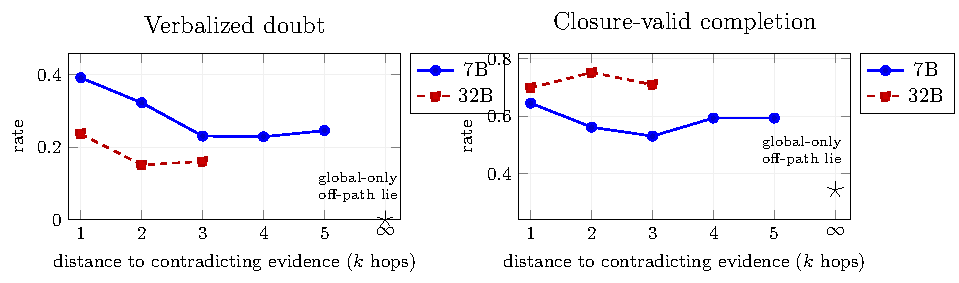
\includegraphics[width=\textwidth]{fig_dose_response.pdf}
\caption{\textbf{The response to a planted lie is a dose--response in inferential
distance.} Negating the fact the model will derive $k$ hops downstream places the
falsifying evidence $k$ inferences from local context. Both verbalized doubt (left)
and validated recovery (right) decline as $k$ grows and then plateau ($k\ge 3$);
globally-checkable-only lies (off-path, $k{\to}\infty$, $\star$) collapse to silent
absorption. 32B shifts the whole curve up rather than steepening it. 7B $n{=}130$
per $k\le3$; $n{=}96,69$ at $k{=}4,5$ (only longer chains admit distant targets).}
\label{fig:dose}
\end{figure}

\subsection{The regime supplies recoverability: three tasks, one protocol}
The same mid-trajectory corruption protocol across task structures (7B):
\begin{center}\small
\begin{tabular}{lccc}
\toprule
Task & Recovery & Absorption & $n$ \\
\midrule
PrOntoQA (redundant derivations) & .53--.86 & .00--.60$^{*}$ & 130/cell \\
GSM8K (natural-language math) & .088 & .877 & 57 \\
Chained arithmetic (no redundancy) & .00--.02 & .99--1.00 & 99/cell \\
\bottomrule
\end{tabular}
\end{center}
($^{*}$The PrOntoQA range is over families; the GSM8K cohort is filtered to the 57 of
250 problems with at least three explicit computations, and the corruption is applied
to the middle one.) The pattern follows how much redundancy each task offers. When
many derivation paths reach the goal, a planted error can be routed around; when every
intermediate is load-bearing, an absorbed error becomes a wrong answer almost every
time. One detail sharpens what ``checkable'' means here: the corrupted GSM8K value
\emph{is} checkable, by a single recomputation --- and it is absorbed anyway. The
checking that produces the PrOntoQA gradient runs over facts \emph{stated in context},
not over arithmetic the model would have to redo. Models re-check what they can
re-read, not what they must recompute. Recoverability is thus a property of the task,
and of how the relevant check must be performed, as much as of the model.

\begin{figure}[t]
\centering
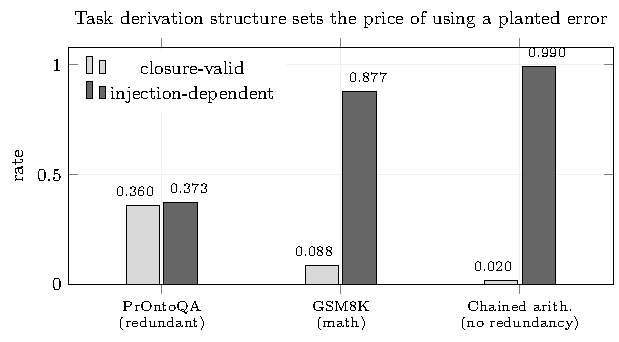
\includegraphics[width=0.62\textwidth]{fig_regime_map.pdf}
\caption{\textbf{Task derivation structure sets the price of an absorbed error.}
A genuine on-path falsehood injected under one protocol across three tasks ordered
by derivation redundancy. As redundant alternative paths disappear (PrOntoQA
$\to$ GSM8K $\to$ chained arithmetic), validated recovery collapses and error
absorption approaches certainty. PrOntoQA is shown with its globally-checkable
(hardest) family for an apples-to-apples comparison with the value corruptions in
GSM8K/arithmetic; its locally-checkable lies recover at .64.}
\label{fig:regime}
\end{figure}

\subsection{Recovery is not goal-anchor re-reading}
Could the apparent recovery be nothing more than the model re-reading the target the
prompt hands it? Two ablations say no. First, we hide the target. Reframing each
problem as ``True or false: $s$?'', with $s$ the true target on half the problems and
its negation on the other half, leaves the statement visible but its truth value
unknown --- so there is no answer to copy. Recovery is attenuated but does not
collapse: 57\% under one-hop falsehoods and 64\% under the benign paraphrase, in a
harder format the model solves only 55\% of the time ($n{=}35/36$). Goal-copying
cannot be the whole story. Second, we tried masking attention to the goal span
directly. This collapses recovery for \emph{both} the falsehood arm (.015) and the
benign arm (.046), which means the manipulation breaks the task itself --- with no
readable target the model has no signal for when its proof is done --- rather than
isolating the recovery mechanism, and we report it as a negative result. Its one usable
finding: with the goal masked, continuations stay chain-sound at the same rate whether
the injection was a falsehood or benign (.45 vs.\ .42), so goal access aids derivation
quality in general, not error recovery in particular.

\subsection{Latent trace}
We also looked for recovery in the hidden states, and report a negative result. Our
metric $\rhofunc_h$ is the Jensen--Shannon divergence between the perturbed and gold
next-token distributions at each sentence boundary, normalized by how far correct
continuations naturally drift (the null ensemble). We verified it against live logits
and confirmed it is instance-specific (a shuffled-gold control gives $1.49\times$
larger divergence). At well-powered horizons (early and mid injection, $h\le 4$,
$n\ge 106$) it shows a clean shape: a spike right after the injection that decays
toward, but stays above, the null band ($\rhofunc_4 \approx 1.2$--$2.3$). The trouble
is that this shape does not track \emph{content}. The benign paraphrase --- a
semantically identical edit --- produces the \emph{largest} early divergence of any
family ($\rhofunc_4 = 2.32$, against 1.9--2.2 for genuine falsehoods), because the
model adopts the injected phrasing for the rest of its proof and the metric reads that
surface change as strongly as a planted lie. As instrumented, $\rhofunc$ cannot tell a
lie from a stylistic tic. Three controls confirm this is real and not an artifact.
Matching the decoding --- sampling perturbed continuations at the null's temperature
($T{=}0.8$, $n{=}4$ per site) --- still leaves benign and falsehood together
($h1$: 22.4 vs.\ 16.3; $h4$: 1.36 vs.\ 1.58), so it is not a greedy-versus-sampled
mismatch. Varying the null ensemble ($T \in \{0.6, 0.8, 1.0\}$, $n \in \{4,8,16,32\}$)
leaves $\rhofunc$ unstable, with medians from 1.9 to 7.9 and interquartile ranges
spanning two orders of magnitude. And the raw geometry agrees: final-layer cosine
divergence is statistically indistinguishable between the benign paraphrase (2.57) and
verified falsehoods (2.52--2.99). Beyond $h{=}2$ for late injections the sample falls
to $n\le 12$ and supports nothing. We therefore make \emph{no} latent claims; the
paper's evidence is behavioral and formally validated. (A token-identity control at
layer 0 was degenerate, since the sentence-boundary token is always a period; a
pooled-sentence version is future work.)

\subsection{Scale attenuates absorption but not silence; the gradient generalizes
across model families}
Running the verified-false families across Qwen2.5 sizes answers the scale
question --- and partially falsifies our pre-registered prediction (we predicted
absorption persists; it persists \emph{attenuated}):
\begin{center}\small
\begin{tabular}{lcccc}
\toprule
 & \multicolumn{3}{c}{globally-checkable falsehood} & 1-hop falsehood \\
Model & valid & poisoned & doubt & doubt \\
\midrule
Qwen2.5-1.5B & .15--.46 & .31--.62 & .000 & .000--.018 \\
Qwen2.5-7B   & .23--.34 & .29--.60 & .000--.057 & .18--.39 \\
Qwen2.5-32B  & .60--.73 & .10--.37 & .033--.067 & .13--.28 \\
\bottomrule
\end{tabular}
\end{center}
Scale buys checking, but not candor. From 7B to 32B, recovery from hard-to-check lies
roughly triples and poisoning roughly halves ($n{=}30$--$35$/cell). The silence,
however, does not move: at every size the lies that get absorbed are absorbed with no
verbalized doubt. (The pre-audit ``wrong-category'' sweep, which is mostly true
interruptions, shows robustness to those rising with scale as well: valid re-derivation
.60--.67 $\to$ .75--.86 $\to$ .88--.96, parroting .11--.20 $\to$ .07--.12 $\to$
.01--.02.)

Two further families separate the behavior from the particular model:
OLMo-2-7B-Instruct (solve rate .69) and Llama-3.1-8B-Instruct. Both reproduce the
\emph{recovery} gradient. At mid injection OLMo recovers benign .72 vs.\ one-hop
falsehood .53, and Llama .79 vs.\ .53, with poisoning in each concentrated in the
globally-checkable family (OLMo .22--.33 at $n{=}9$; Llama recovery collapsing to
.22--.26 with poisoning .41--.44 at $n{=}27$; $n{=}76$ and $107$ per cell for the
well-powered families). Neither \emph{flags}: both voice essentially no doubt in any
family (OLMo .00--.026, Llama .00--.009), recovering from checkable lies as silently as
the 1.5B Qwen does. So the checkability gradient in \emph{behavior} is model-general
across three lineages, while \emph{verbalizing} a caught error is not; recovery does not
require the model to say anything. (We also attempted Mistral-7B-Instruct, but it does
not produce the parseable proof grammar these tasks require --- too few continuations
had valid injection points to analyze --- and we exclude it.)

DeepSeek-R1-Distill-Qwen-7B isolates the training axis: the same 7B backbone, plus
reasoning RL. (We inject into the visible proof and strip the think block before
validating; the model solves 29\% of problems and leaves 8--16\% of runs unparsed,
which we report as-is.) Our pre-registered prediction --- doubt rises, recovery stays
flat --- holds. Visible flagging of one-hop falsehoods reaches .672 ($n{=}122$),
against .25 for Qwen-7B and .00 for OLMo, while validated recovery barely moves
(.689 vs.\ .638), and the flagging is selective --- only .008 on the benign paraphrase.
Read across all five models, the picture is a spectrum --- silent (OLMo, 1.5B),
moderate (7B, 32B), loud (R1) --- at roughly constant recovery. \emph{Flagging is
trained; recovery is intrinsic.} (R1's hidden reasoning channel is uninformative here,
since every gold think block already contains doubt words --- a ceiling. R1 also
handles the benign paraphrase \emph{worse} than its base model, .549 vs.\ .815:
reasoning training buys verbalization at some cost in robustness to mere disruption.)

\begin{figure}[t]
\centering
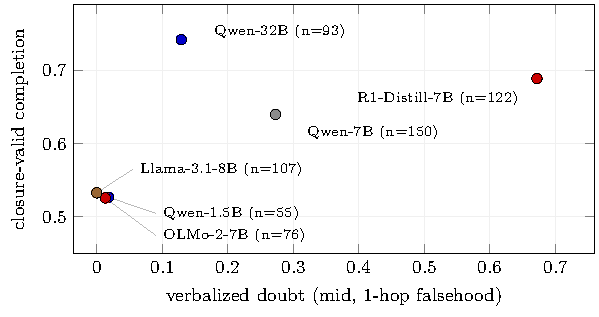
\includegraphics[width=0.66\textwidth]{fig_verbalization_spectrum.pdf}
\caption{\textbf{Verbalization is trained; recovery is intrinsic.} Across five models
(1-hop falsehood, mid injection), verbalized doubt ranges over $50\times$ (.01 to .67)
while validated recovery stays within a narrow band (.53--.74). Reasoning-RL training
(R1-Distill) buys loud flagging at flat recovery; the base/instruct models recover at
comparable rates while saying nothing. Verbalizing a caught error and correcting it
are dissociable behaviors.}
\label{fig:verbal}
\end{figure}

\section{Limitations}
Our coverage is still narrow. The tasks are two synthetic families plus GSM8K, whose
cohort is filtered to the 57 of 250 problems with at least three explicit steps; a
formal-verification task such as Lean is the natural next regime. The models span three
sizes, a second family (OLMo-2), and a reasoning-RL variant (R1-Distill), but remain
largely one lineage. We use deterministic decoding and a single null-sampling seed. The
globally-checkable falsehood family --- the one that produces silent absorption --- has
only $n{=}35$ per cell and exists for about 30\% of problems, though a within-subset
control rules out instance selection; the QA-format condition is similarly small
($n{=}35$--$36$). We operationalize ``local falsifiability'' at two levels
(contradiction-distance zero to one, versus global) and report a three-point distance
curve; a fully parametric version is future work. The prompt states the proof target,
which the validator's parroting category and the goal-hidden QA condition address,
though goal-directedness may still aid derivation quality in general. Our latent and
geometric metrics are negative results. And closure-based validation permits
step-skipping, which we quantify (4.7--9.2\%) rather than eliminate.

\section{Related work}
\textbf{CoT interventions and error recovery.} \citet{vonrecum2026robust} perturb
visible CoT in reasoning-tuned models and find behavioral robustness with
early-intervention degradation and doubt/length effects, on free-form reasoning where
our entailment-based construction does not directly apply. \citet{yee2024dissociation}
precede our re-derivation/parroting split with a faithful/unfaithful recovery
dichotomy via manual annotation; our delta is automated formal validation, semantic
(vs.\ numerical) error control, and the falsifiability gradient. Their finding that recovery is more frequent for \emph{obvious} errors
independently anticipates checkability-gating. \citet{lanham2023measuring} introduced
adding-mistakes interventions for faithfulness; \citet{turpin2023unfaithful} showed
stated reasoning can omit operative causes --- consistent with silent absorption.
\citet{zhang2023snowball} showed models commit to early mistakes they can separately
recognize; our results locate when that recognition is and is not deployed in-rollout.
\citet{huang2024cannot} found intrinsic self-correction weak at the multi-turn level;
silent absorption is its single-pass analogue, while flagging shows the capacity
exists when the check is local.
\textbf{Self-repair and redundancy.} \citet{mcgrath2023hydra,lad2024stages} document
structural self-repair; silent absorption is the complementary failure: robustness
machinery that smooths over content errors it cannot cheaply check.
\textbf{Trajectory geometry.} \citet{sun2026trajectories} characterize reasoning as
step-specific representational trajectories with correctness signals; our
style-propagation result (benign $\approx$ falsehood in both functional and geometric
divergence) is a caution for cross-trace comparisons in that line.
\textbf{Compounding.} \citet{dziri2023faith,lecun2022path} supply the ingredients of
the compounding frame our results sharpen: per-step absorption is real exactly when
errors are locally unfalsifiable, and task derivation structure (\S5.3) determines
the price.
\textbf{Verification benchmarks.} External-verifier and formally-checkable benchmarks
complement our internal-only framing. VerifyBench \citep{verifybench2025} evaluates
reference-based reward verifiers, while VERINA \citep{verina2025} and VeriBench
\citep{veribench2026} score end-to-end verifiable code and proof generation in Lean.
Most directly, VeriSoftBench \citep{verisoftbench2026} reports that repository-scale
proof success falls as a task's \emph{transitive dependency closure} grows --- a
structural echo, in a real Lean regime, of our finding that the errors that go uncaught
are precisely the globally-checkable ones. Such formal settings, where global checks are
structurally unavoidable, are the natural place to test whether silent absorption
persists once the verifier is external rather than the model itself.

\section*{Reproducibility}
Single 8$\times$H200 node, $\sim$8 GPU-hours total. Pre-registered plan
(\texttt{PLAN.md}, written before the first run), all scripts, per-run JSONL logs,
and result JSONs accompany the paper
(\texttt{experiments/09\_latent\_recovery/}).

\bibliographystyle{plainnat}
\begin{thebibliography}{9}
\bibitem[VerifyBench(2025)]{verifybench2025}
VerifyBench: Benchmarking Reference-based Reward Systems for Large Language Models.
arXiv:2505.15801, 2025.
\bibitem[VERINA(2025)]{verina2025}
VERINA: Benchmarking Verifiable Code Generation. arXiv:2505.23135, 2025.
\bibitem[VeriBench(2026)]{veribench2026}
VeriBench: End-to-End Formal Verification Benchmark for AI Code Generation in Lean 4.
OpenReview, 2026.
\bibitem[VeriSoftBench(2026)]{verisoftbench2026}
VeriSoftBench: Repository-Scale Formal Verification Benchmarks for Lean.
arXiv:2602.18307, 2026.
\bibitem[Dziri et al.(2023)]{dziri2023faith} N. Dziri et al.
\newblock Faith and Fate: Limits of Transformers on Compositionality.
\newblock \emph{NeurIPS}, 2023. arXiv:2305.18654.
\bibitem[Lad et al.(2024)]{lad2024stages} V. Lad, J.H. Lee, W. Gurnee, M. Tegmark.
\newblock The Remarkable Robustness of LLMs: Stages of Inference?
\newblock arXiv:2406.19384, 2024.
\bibitem[LeCun(2022)]{lecun2022path} Y. LeCun.
\newblock A Path Towards Autonomous Machine Intelligence. OpenReview, 2022.
\bibitem[McGrath et al.(2023)]{mcgrath2023hydra} T. McGrath et al.
\newblock The Hydra Effect: Emergent Self-repair in Language Model Computations.
\newblock arXiv:2307.15771, 2023.
\bibitem[Saparov and He(2023)]{saparov2023prontoqa} A. Saparov and H. He.
\newblock Language Models Are Greedy Reasoners: A Systematic Formal Analysis of
Chain-of-Thought. \emph{ICLR}, 2023. arXiv:2210.01240.
\bibitem[Yee et al.(2024)]{yee2024dissociation} E. Yee, A. Li, C. Tang, Y.H. Jung,
R. Paturi, L. Bergen.
\newblock Dissociation of Faithful and Unfaithful Reasoning in LLMs.
\newblock arXiv:2405.15092, 2024.
\bibitem[Lanham et al.(2023)]{lanham2023measuring} T. Lanham et al.
\newblock Measuring Faithfulness in Chain-of-Thought Reasoning.
\newblock arXiv:2307.13702, 2023.
\bibitem[Turpin et al.(2023)]{turpin2023unfaithful} M. Turpin, J. Michael,
E. Perez, S. Bowman.
\newblock Language Models Don't Always Say What They Think.
\newblock \emph{NeurIPS}, 2023. arXiv:2305.04388.
\bibitem[Zhang et al.(2023)]{zhang2023snowball} M. Zhang, O. Press, W. Merrill,
A. Liu, N.A. Smith.
\newblock How Language Model Hallucinations Can Snowball.
\newblock arXiv:2305.13534, 2023.
\bibitem[Huang et al.(2024)]{huang2024cannot} J. Huang et al.
\newblock Large Language Models Cannot Self-Correct Reasoning Yet.
\newblock \emph{ICLR}, 2024. arXiv:2310.01798.
\bibitem[Sun et al.(2026)]{sun2026trajectories} L. Sun, H. Dong, B. Qiao, Q. Lin,
D. Zhang, S. Rajmohan.
\newblock LLM Reasoning as Trajectories: Step-Specific Representation Geometry and
Correctness Signals.
\newblock arXiv:2604.05655, 2026.
\bibitem[von Recum et al.(2026)]{vonrecum2026robust} A. von Recum, L. Girrbach,
Z. Akata.
\newblock Are Reasoning LLMs Robust to Interventions on Their Chain-of-Thought?
\newblock arXiv:2602.07470, 2026.
\end{thebibliography}

\end{document}
